% Compile with LuaLaTeX or XeLaTeX
\documentclass[11pt,a4paper,twocolumn]{article}

% Required Packages
\usepackage[utf8]{inputenc}
\usepackage[english]{babel}
\usepackage[T1]{fontenc}
\usepackage[usefilenames,DefaultFeatures={Ligatures=Common}]{plex-otf}
\usepackage{fontspec}
\usepackage{graphicx}
\usepackage{float} % To control figure placement with [H]
\usepackage{hyperref}
\usepackage{amsmath}
\usepackage{parskip}
\usepackage{titlesec}
\usepackage[margin=1in,columnsep=0.25in]{geometry}
\usepackage{titling}
\usepackage{microtype}
\usepackage{balance}
\bibliographystyle{plain}

% Font Configurations
\setmainfont{IBM Plex Serif} % Main body font
\setsansfont{IBM Plex Sans}  % Title, author, and figure captions
\setmonofont{IBM Plex Mono} % Section titles and subsections

% Adjust Title and Section Formatting
\titleformat{\section}[block]{\large\bfseries\ttfamily}{\thesection}{1em}{} % IBM Plex Mono for sections
\titlespacing*{\section}{0pt}{2em}{1em}
\titleformat{\subsection}[runin]{\bfseries\ttfamily}{\thesubsection}{0.5em}{} % IBM Plex Mono for subsections
\titlespacing*{\subsection}{0pt}{1em}{0.5em}
\setlength{\droptitle}{-1cm} % Adjust title position
\raggedbottom % Prevent uneven stretching

% Document Information
\title{\ttfamily Executive Summary: Addressing the Challenges of Server Virtualization} % IBM Plex Mono for title
\author{\sffamily Izaac Plambeck \\ (SysAdmin)} % IBM Plex Sans for author
\date{\sffamily January 19, 2025} % IBM Plex Sans for manually set date

\begin{document}

% Title
\twocolumn[
\begin{@twocolumnfalse}
\maketitle
\end{@twocolumnfalse}
]

% Executive Summary Section
\section{Executive Summary: Addressing the Challenges of Server Virtualization}
As the system administrator for our organization, tasked with evaluating the feasibility of server virtualization, it is imperative to highlight potential disadvantages to ensure a comprehensive understanding of its risks. This summary focuses on \textbf{Virtual Machine (VM) sprawl}, a critical challenge that arises when virtualized environments are not carefully managed.

% What is VM Sprawl Section and Image
\begin{figure}[H] % Use float package to control placement
    \centering
    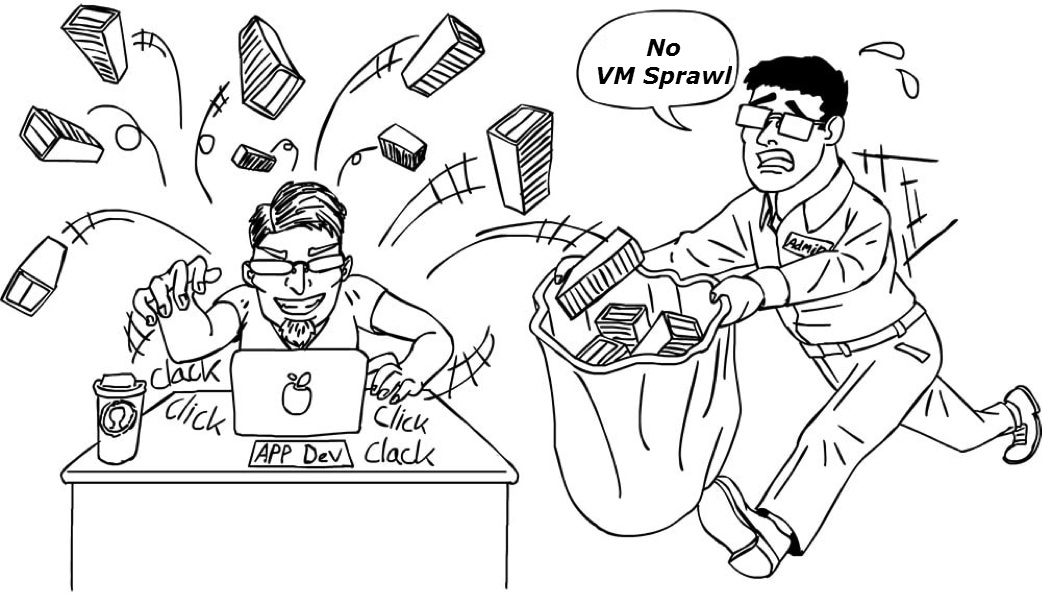
\includegraphics[width=0.8\linewidth]{novmsprawl.png}
    \caption{\sffamily Illustration of Virtual Machine (VM) Sprawl Costing Us Money} % IBM Plex Sans for figure caption
    \label{fig:vm_sprawl}
\end{figure}

\section{What is VM Sprawl?}
VM sprawl refers to the uncontrolled proliferation of virtual machines within a virtualized server environment. This phenomenon often occurs when VMs are created easily but without proper lifecycle management. Over time, this leads to an overwhelming number of VMs, many of which are underutilized or redundant.

The ease of VM creation, while beneficial for agility, can result in unchecked growth, creating challenges that impact resource allocation, operational efficiency, and security.

% Why is VM Sprawl a Potential Disadvantage?
\section{Why is VM Sprawl a Potential Disadvantage?}
The uncontrolled expansion of VMs introduces three primary risks:

\subsection{Wasted Resources}
Underutilized VMs unnecessarily consume critical resources like CPU, memory, and storage. These inefficiencies strain infrastructure, reduce the capacity for productive workloads, and increase operational costs.

\subsection{Increased Management Complexity}
A growing number of VMs complicates lifecycle management, making it difficult to track, monitor, and decommission instances effectively. This increases administrative overhead and reduces overall system efficiency.

\subsection{Heightened Security Vulnerabilities}
Forgotten or under-monitored VMs can miss essential updates and patches, creating exploitable vulnerabilities. The expanded attack surface leaves the organization susceptible to cyber threats, undermining the security of the virtualized infrastructure.

% Strategies to Mitigate VM Sprawl
\section{Strategies to Mitigate VM Sprawl}
To effectively address VM sprawl, the following actionable measures are recommended:

\subsection{Automate VM Management}
Leverage tools to automate the provisioning, monitoring, and decommissioning of VMs. Automation minimizes manual oversight errors, ensures compliance, and prevents the unchecked growth of virtual instances.

\subsection{Enforce Governance Policies}
Establish clear policies that regulate VM creation and resource allocation. Implement approval workflows and usage quotas to ensure the environment remains balanced and efficient.

\subsection{Monitor and Audit Regularly}
Utilize monitoring tools to track VM performance, identify underused or redundant machines, and decommission those that no longer serve a purpose. Conducting periodic audits ensures resource reclamation and optimization.

\subsection{Provide Staff Training}
Equip IT staff with the knowledge and tools necessary to recognize and manage VM sprawl proactively. Training ensures that the team is aligned with best practices for maintaining virtualized environments.

% Conclusion
\section{Conclusion}
As we evaluate the benefits of server virtualization, addressing VM sprawl is vital to maintaining a cost-effective, efficient, and secure infrastructure. By implementing robust automation, governance, monitoring, and training, our organization can mitigate the risks associated with VM sprawl and optimize the advantages of virtualization.

% References
\section{References}
\begin{enumerate}
    \item Miller, L. C., \emph{Server Virtualization for Dummies}. Oracle Special Edition.
    \item Portnoy, M., \emph{Virtualization Essentials}.
\end{enumerate}

\end{document}
